\documentclass[a4paper, 12pt]{article}
\usepackage[UTF8]{ctex}
\usepackage{geometry}
\usepackage{graphicx}
\usepackage{float}
\usepackage{hyperref}

% 设置页边距
\geometry{a4paper, left=2.5cm, right=2.5cm, top=2.5cm, bottom=2.5cm}

\begin{document}

\title{\huge{系统开发工具基础实验报告}}
\author{姓名:\underline{刘浩洋} \\ 
        学号:\underline{24040021022} \\ 
        班级:\underline{软件工程}}
\date{实验日期:\underline{2025年8月29日}}
\maketitle

\section*{一、实验目的}
本次实验旨在通过学习和实践 LaTeX 和 Git 的基本使用方法,掌握以下技能:
\begin{itemize}
    \item 掌握 LaTeX 文档的基本结构和常用命令。
    \item 理解并应用 Git 进行版本控制,包括创建仓库、提交修改、查看历史记录等操作。
    \item 完成指定任务,如编写简单的 LaTeX 文档和管理代码项目。
\end{itemize}

\section*{二、实验环境}
为了完成本次实验,需要以下软硬件环境:
\begin{itemize}
    \item 操作系统:Windows 11
    \item 软件工具:
    \begin{itemize}
        \item Overleaf(用于在线编辑 LaTeX 文档)
        \item Git for Windows(用于本地 Git 操作)
    \end{itemize}
\end{itemize}

\section*{三、练习内容}
本次实验要求完成以下任务:
\begin{enumerate}
    \item 在 Overleaf 中创建一个简单的 LaTeX 文档,并添加标题、作者信息、章节等内容。
    \item 使用 Git 创建一个新的本地仓库,并进行初始化、添加文件、提交修改等操作。
    \item 将本地仓库推送到 GitHub 上的远程仓库。
\end{enumerate}

\section*{四、实验过程}
以下是详细的实验步骤:

\begin{enumerate}
    \item \textbf{搭建环境}
    \begin{itemize}
        \item 注册并登录 Overleaf,创建新项目。
        \item 安装 Git for Windows,并配置用户名和邮箱。
    \end{itemize}

    \item \textbf{编写 LaTeX 文档}
    \begin{itemize}
        \item 在 Overleaf 中创建一个新的 LaTeX 项目,选择合适的文档类(如 `article`)。
        \item 添加标题、作者、日期等信息,并插入图片等元素。
        \item 编译文档,检查输出是否符合预期。
    \end{itemize}

    \begin{figure}[htbp]
        \centering
        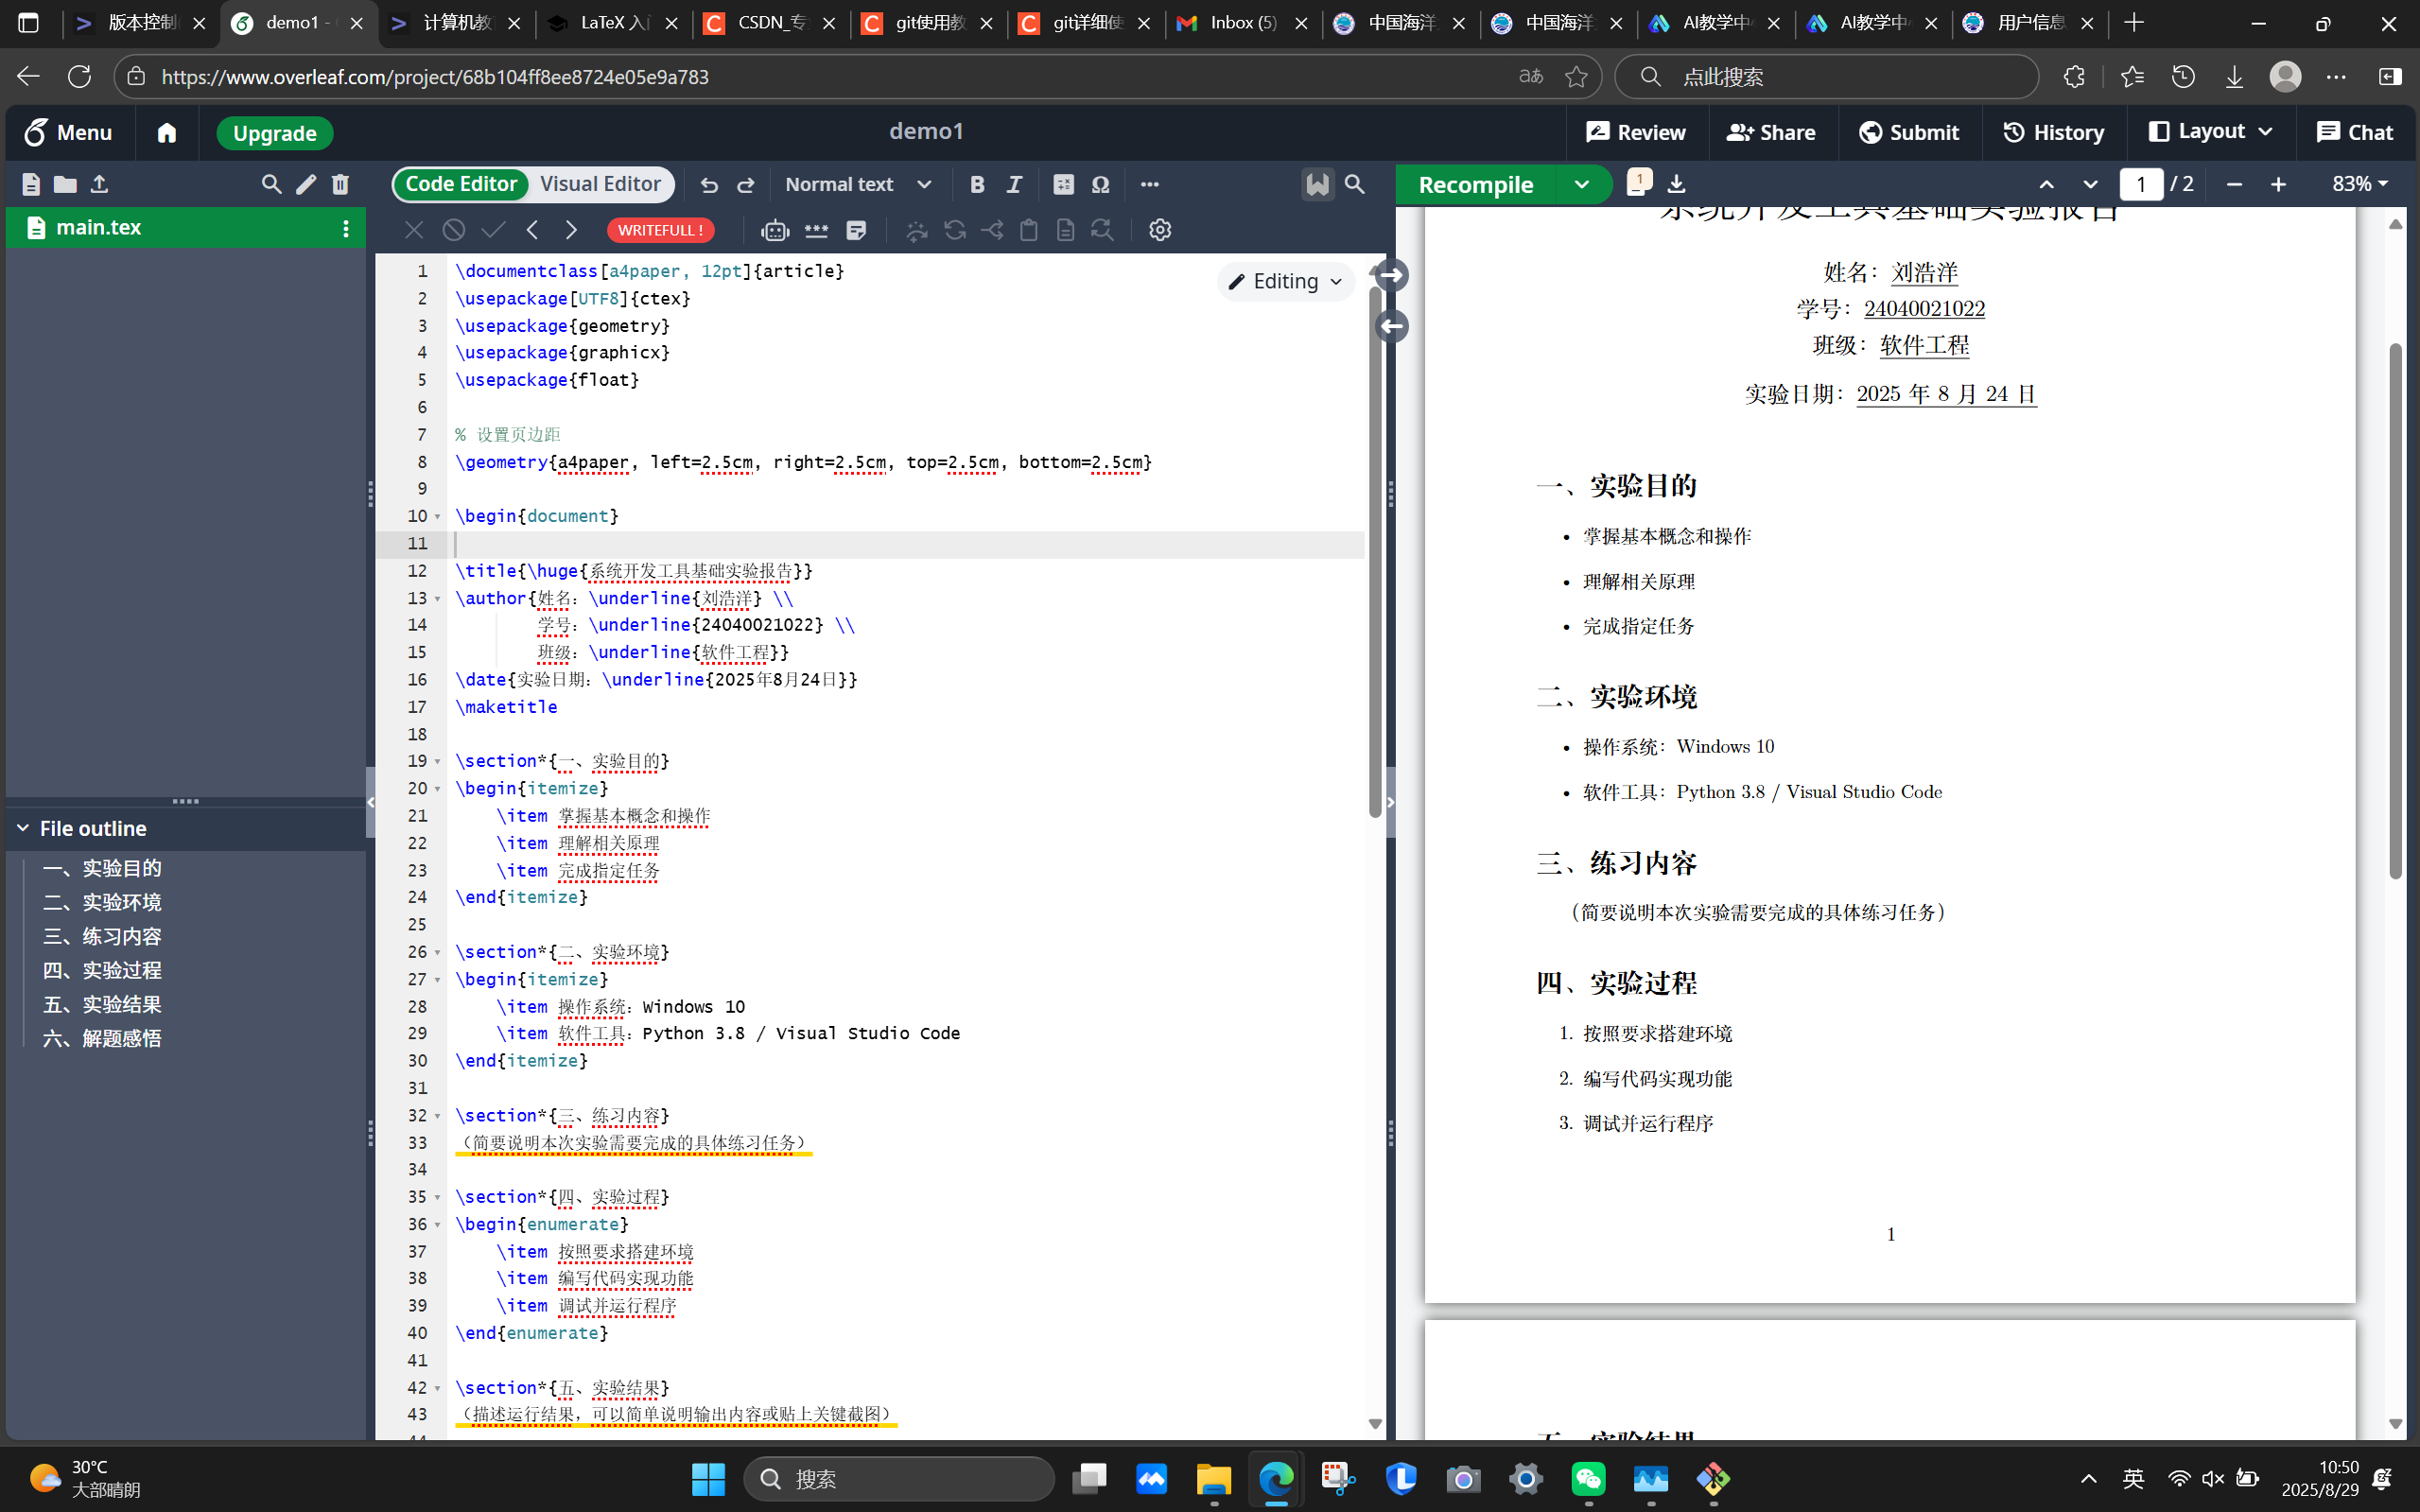
\includegraphics[width=0.8\textwidth]{latex.png}%0.8倍文本宽度
        \caption{LaTeX 文档编译结果截图}
        \label{fig:latex}
    \end{figure}

    \item \textbf{使用 Git 进行版本控制}
    \begin{itemize}
        \item 在本地创建一个新的 Git 仓库,并初始化。
        \item 添加实验报告文件到暂存区,并提交修改。
        \item 查看提交历史,确保所有修改都被正确记录。
    \end{itemize}
    
    \begin{figure}[htbp]
        \centering
        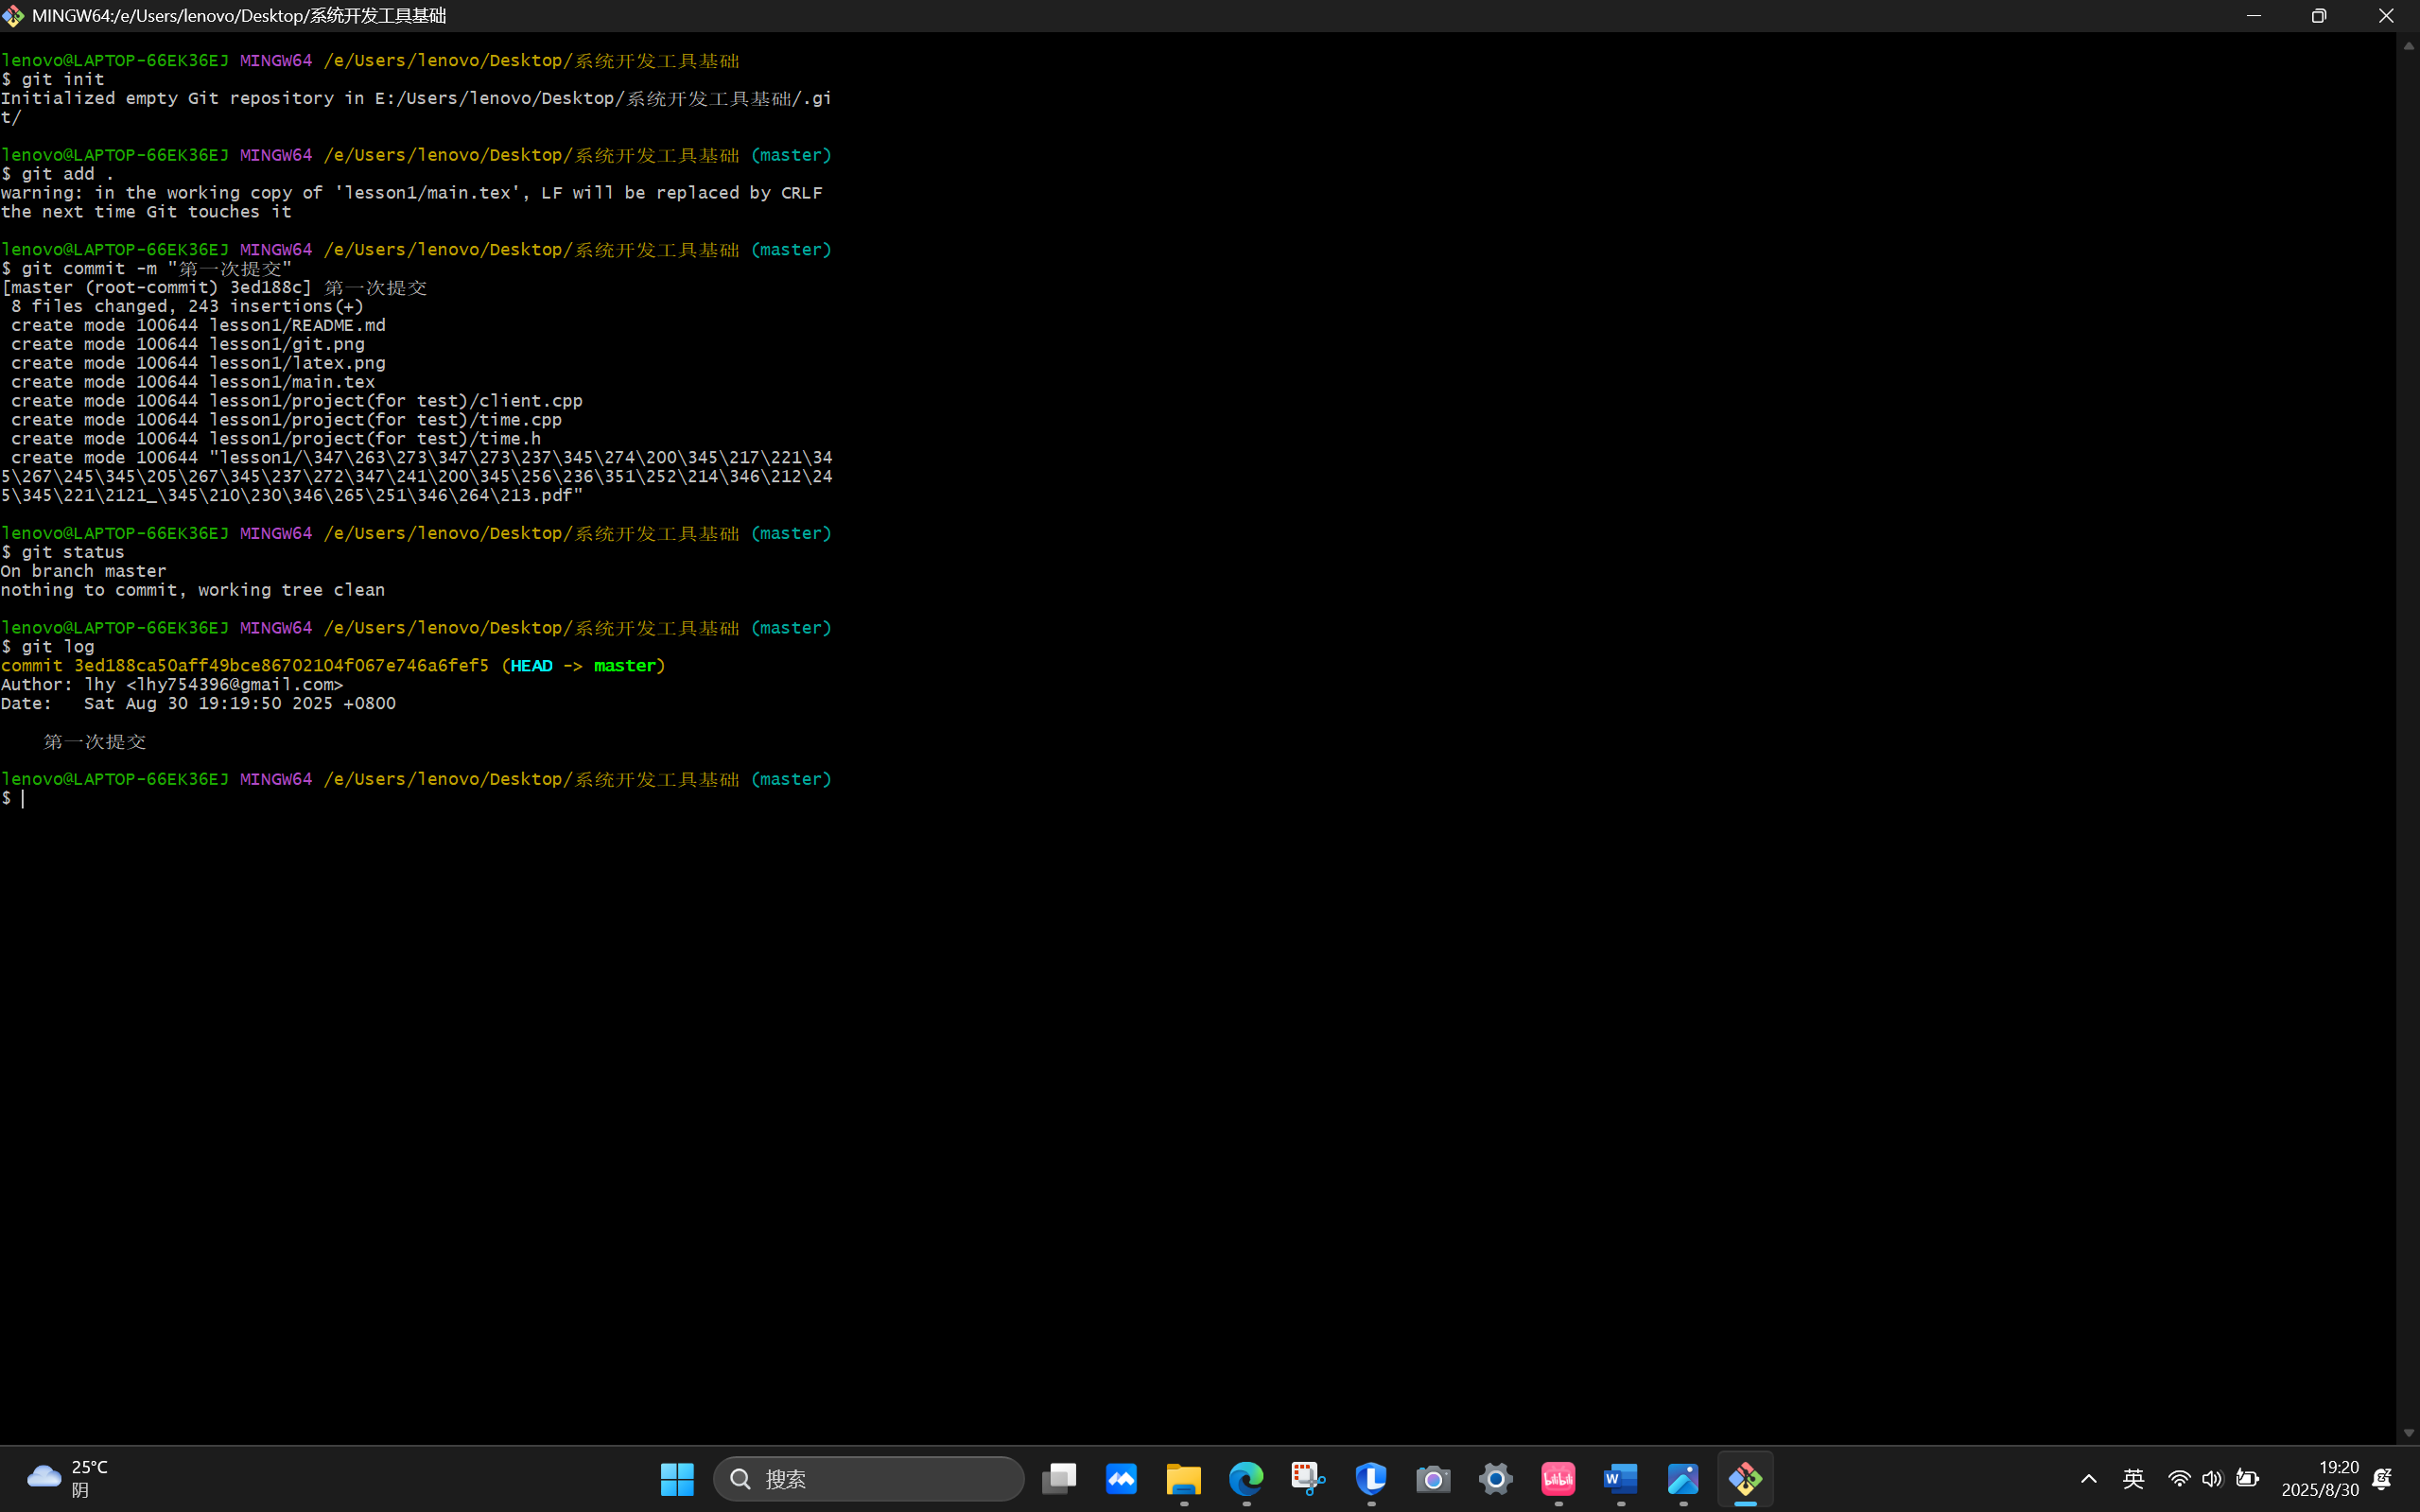
\includegraphics[width=0.8\textwidth]{git1.png}%0.8倍文本宽度
        \caption{Git 基本操作截图}
        \label{fig:git1}
    \end{figure}
    
    \item \textbf{推送至远程仓库}
    \begin{itemize}
        \item 登录 GitHub,创建一个新的远程仓库。
        \item 将本地仓库与远程仓库关联,并推送代码。
        \item 邀请同学或老师加入协作,共同编辑和提交修改。
    \end{itemize}
    
    \begin{figure}[htbp]
        \centering
        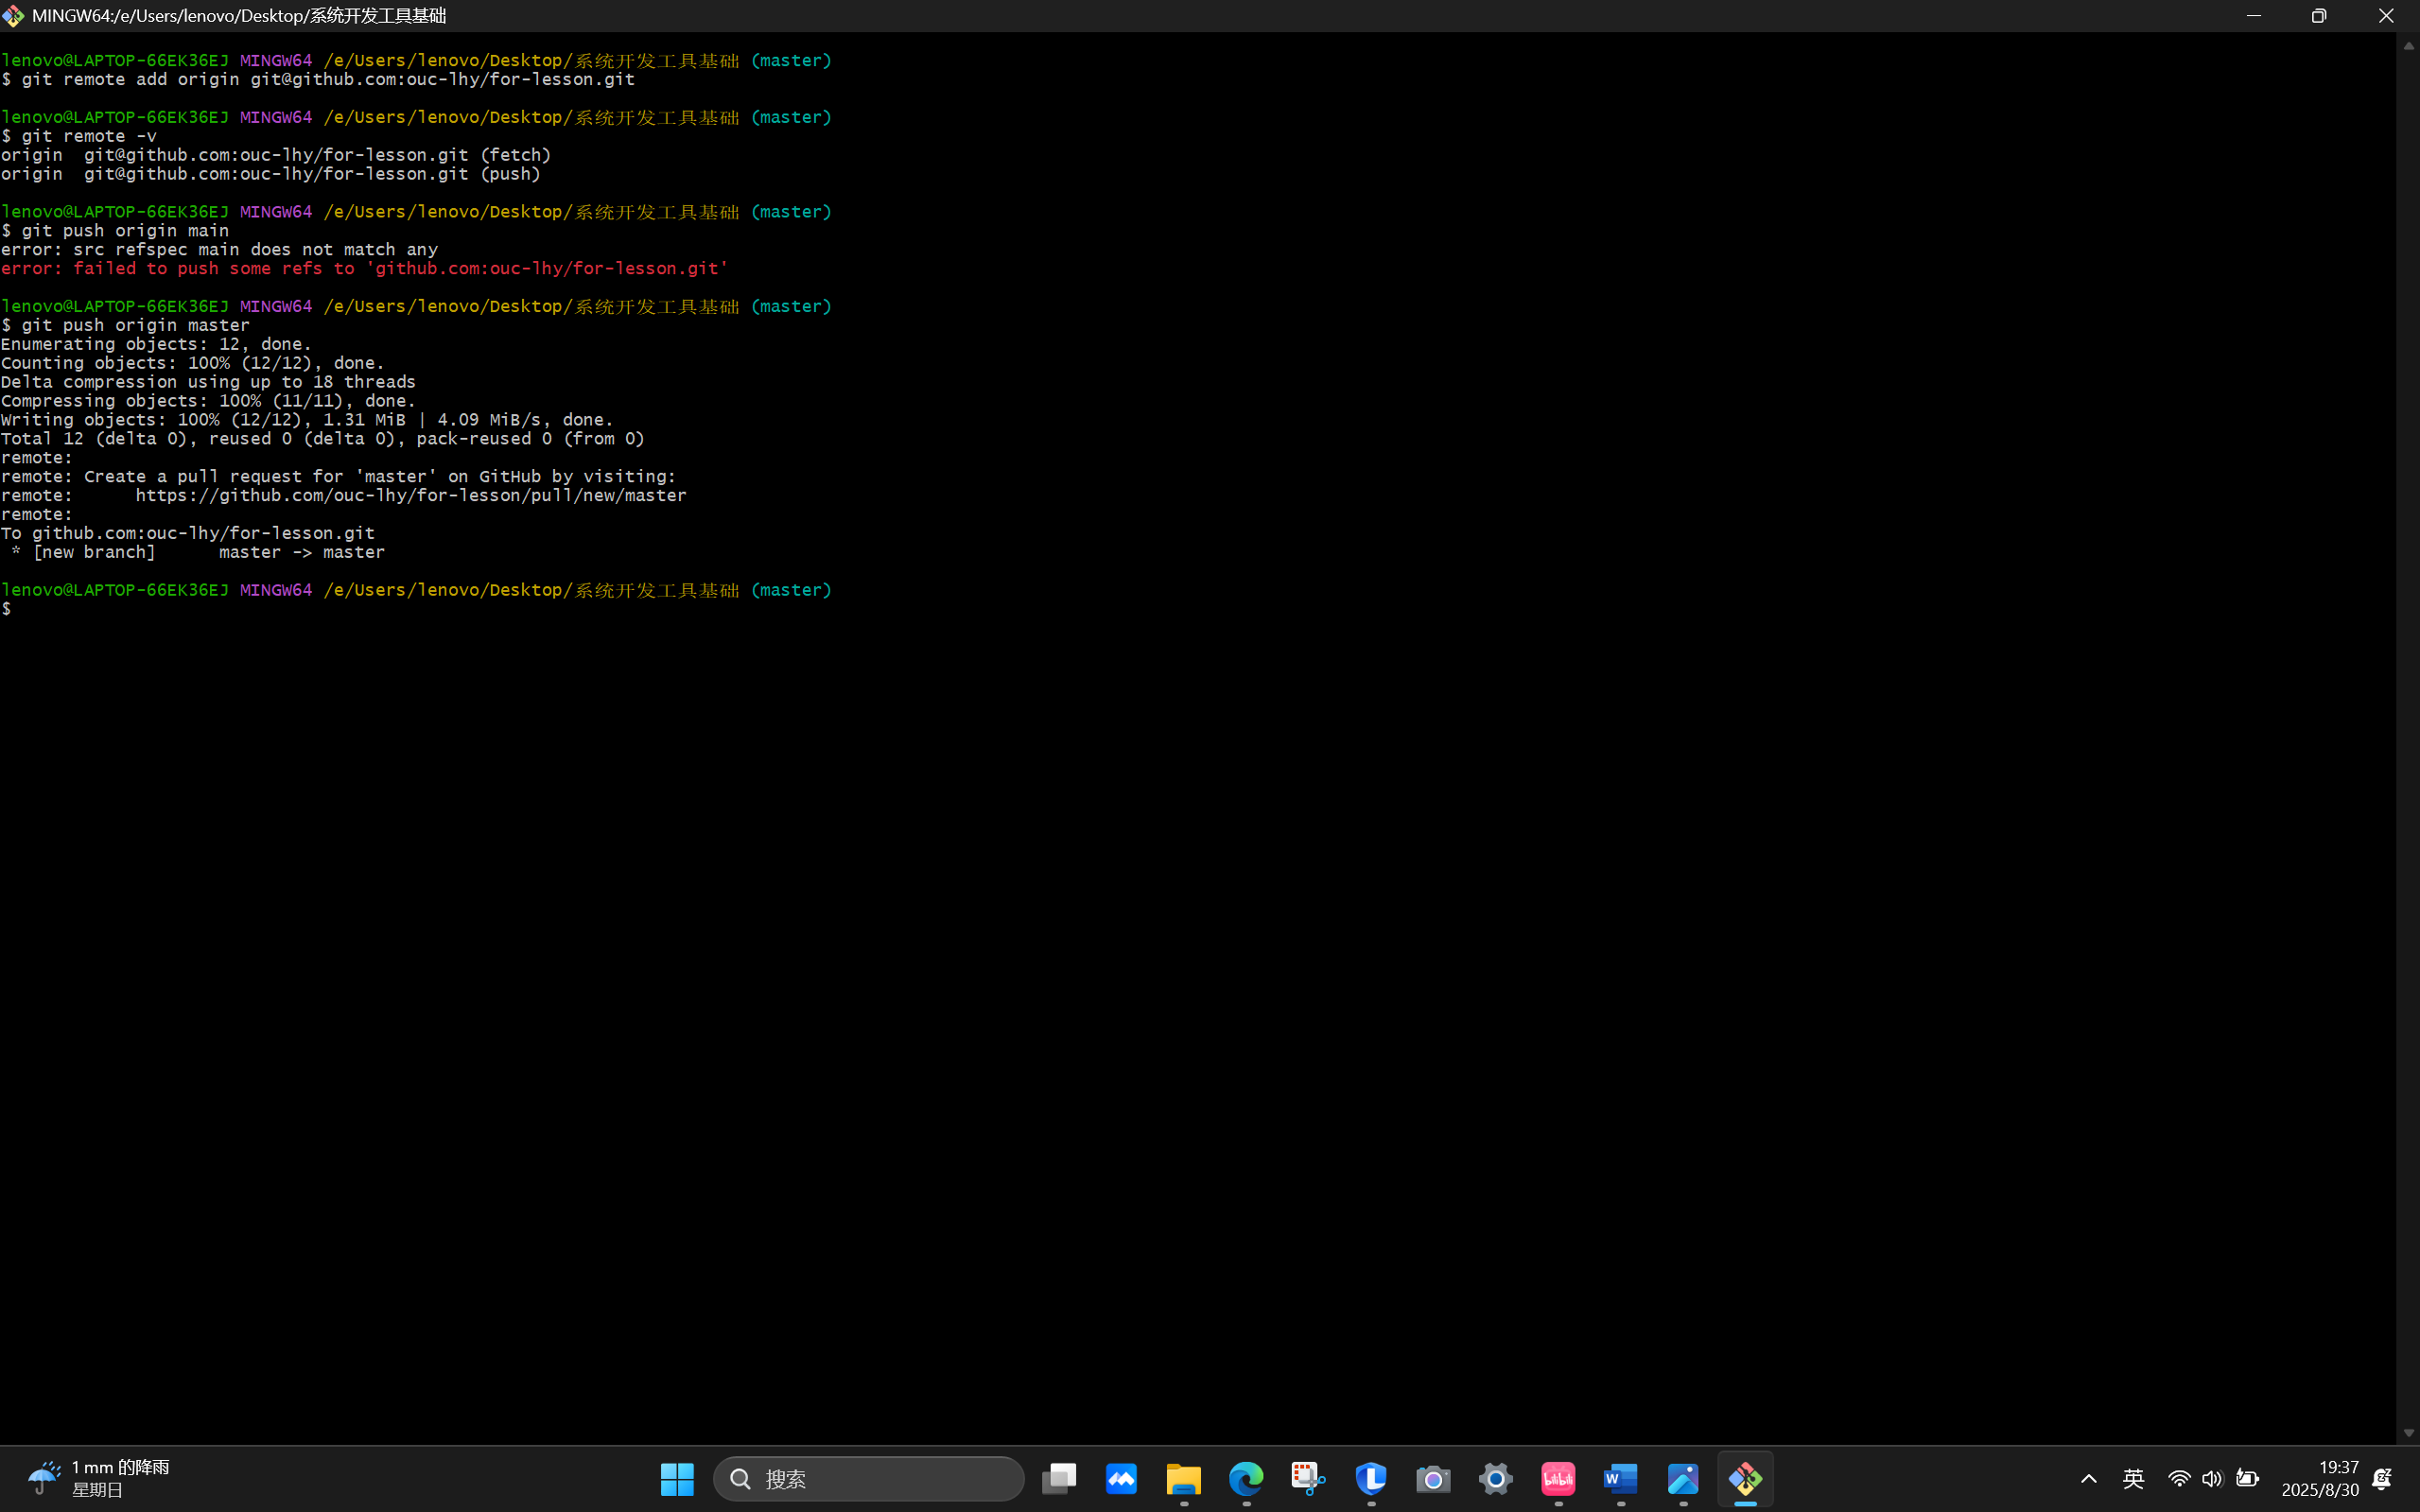
\includegraphics[width=0.8\textwidth]{git2.png}%0.8倍文本宽度
        \caption{Git 基本操作截图}
        \label{fig:git2}
    \end{figure}
    
\end{enumerate}

\section*{五、实验结果}
在本次实验中,成功完成了以下任务:
\begin{itemize}
    \item 创建了一个简单的 LaTeX 文档,并实现了标题、作者信息、章节、图片等元素的插入。图 \ref{fig:latex} 展示了最终编译后的效果。
    \item 使用 Git 进行了版本控制,创建了本地仓库并进行了多次提交。图 \ref{fig:git1}和图 \ref{fig:git2} 显示了 Git 的基本操作界面。
    \item 成功将本地仓库推送到 GitHub 远程仓库\url{https://github.com/ouc-lhy/for-lesson/tree/master/lesson1}
\end{itemize}

\section*{六、解题感悟}
通过本次实验,我深入了解了 LaTeX 文档的编写流程和 Git 版本控制的基本操作。具体收获如下:
\begin{itemize}
    \item LaTeX 是一种非常强大的排版工具,特别适合学术论文和技术文档的撰写。通过这次实验,掌握了如何编写结构化的文档,以及如何插入图片、表格和公式等元素。
    \item Git 提供了高效的版本控制功能,能够帮助开发者更好地管理代码变更。通过实际操作,熟悉了 Git 的常见命令,如 `git init`, `git add`, `git commit`, `git push`,`git pull` 等,提升了对版本控制的理解。
\end{itemize}

\section*{七、github链接}

本次实验的代码和文档可以在 GitHub 上找到:\url{https://github.com/ouc-lhy/for-lesson/tree/master/lesson1} 或者直接点击 \href{https://github.com/ouc-lhy/for-lesson/tree/master/lesson1}{这里} 查看。

\end{document}